%__________________________________________________________________________________

\chapter{Synchronization Extremes: Free and Always-Synchronizing LTNs}
\label{chap:fragments}

Chapter~\ref{chap:ltn} showed that location reachability is undecidable for general
local-timed negotiations. The proof of Theorem~\ref{thm:undecidability} identified
two features whose interaction is essential for this result:

\begin{enumerate}
\item \emph{Unbounded clock drift}: the reference clocks $t_p$ and $t_q$ of different
agents may diverge arbitrarily, allowing the encoding of unbounded integer values.
\item \emph{Explicit synchronization}: synchronizing nodes require equality of
reference clocks, enabling the system to compare and condition behavior on
accumulated drift.
\end{enumerate}

It is precisely the combination of these two mechanisms—arbitrary accumulation
of drift and the ability to test it—that yields the expressive power of counter
machines. Part~II explores how decidability can be recovered by restricting one
or both of these sources of power.

This chapter focuses on the first axis of restriction, namely synchronization.
Rather than allowing arbitrary mixtures of synchronizing and non-synchronizing
nodes, we study the two extreme regimes:
\begin{itemize}
\item \textbf{Synchronization-free LTNs} ($\text{Sync} = \emptyset$), where no node
imposes equality of reference clocks and agents evolve completely independently.
\item \textbf{Always-synchronizing LTNs} ($\text{Sync} = N$), where every interaction
requires temporal alignment of participating agents.
\end{itemize}

In both cases, the critical interaction between unbounded drift and synchronization
is eliminated, albeit in opposite ways. As a consequence, location reachability
becomes decidable.

\paragraph{Conceptual role of the extremes.}
In these two fragments, we recover decidability by removing the interplay between drift and synchronization. Understanding why these extremes are decidable clarifies which features cause undecidability in the general model.
Despite of having the same worst-case complexity, the two fragments require
fundamentally different proof techniques. Synchronization-free LTNs admit a
componentwise abstraction that exploits the complete independence of agents,
whereas always-synchronizing LTNs collapse to a global-time semantics and can be
reduced to classical timed automata.

\paragraph{Main results.}
The central results of this chapter are the following.

\begin{theorem}[Chapter results]
\label{thm:chapter-results}
Location reachability is PSPACE-complete for each of the following classes:
\begin{enumerate}
\item synchronization-free local-timed negotiations (Section~\ref{sec:syncfree});
\item always-synchronizing local-timed negotiations (Section~\ref{sec:always-sync}).
\end{enumerate}
\end{theorem}

In both cases, the complexity matches that of reachability for timed automata.
Thus, while these fragments do not exploit the negotiation structure to reduce
complexity, they also do not incur additional algorithmic cost beyond what is
inherent to quantitative timing.

\paragraph{Organization.}
Section~\ref{sec:syncfree} studies synchronization-free LTNs via a product-style
region abstraction. Section~\ref{sec:always-sync} analyzes always-synchronizing
LTNs by reducing them to a global-time model. Section~\ref{sec:fragments-synthesis}
synthesizes the lessons from both extremes, and Section~\ref{sec:fragments-next}
positions them within the broader landscape of decidable fragments studied in
subsequent chapters.

%__________________________________________________________________________________
%%%%%%%%%%%%%%%%%%%%%%%%%%%%%%%%%%%%%%%%%%%%%%%%%%%
\begin{comment}
\section{A Running Example}
\paragraph{A running example.}
The following simple two-agent LTN will be used to illustrate the proof techniques for synchronization-free and always-synchronizing LTNs.

Let $P = \{p,q\}$. Each agent has one local clock:
$X_p = \{x\}$ and $X_q = \{y\}$.
The negotiation has three nodes: $N = \{n_0, n_1, n_2\}$
with domains: $\text{dom}(n_0) = \{p,q\}, 
\text{dom}(n_1) = \{p\}, 
\text{dom}(n_2) = \{p,q\}.$

\begin{figure}[t]
\centering

% --- Diagram 1: Synchronization-Free Semantics ---
\begin{subfigure}[b]{0.45\textwidth}
\centering
\resizebox{\textwidth}{!}{%
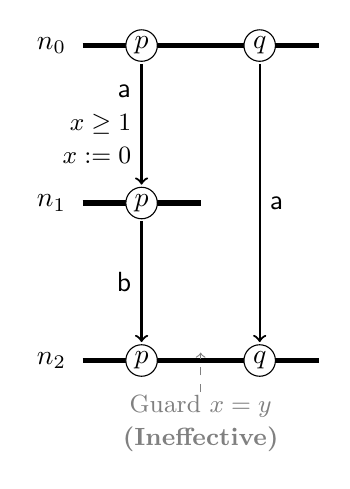
\begin{tikzpicture}
    % Nodes (Bars)
    \draw[line width=2pt] (0,4) node[left] {$n_0\,$} -- (3,4);
    \draw[line width=2pt] (0,2) node[left] {$n_1\,$} -- (1.5,2);
    \draw[line width=2pt] (0,0) node[left] {$n_2\,$} -- (3,0);

    % Ports
    \filldraw[fill=white] (0.75,4) circle (2mm) node (p_n0) {$p$};
    \filldraw[fill=white] (2.25,4) circle (2mm) node (q_n0) {$q$};
    
    \filldraw[fill=white] (0.75,2) circle (2mm) node (p_n1) {$p$};
    
    \filldraw[fill=white] (0.75,0) circle (2mm) node (p_n2) {$p$};
    \filldraw[fill=white] (2.25,0) circle (2mm) node (q_n2) {$q$};

    % Edges
    % p: n0 -> n1
    \draw[->, thick] (p_n0) -- (p_n1) node[midway, left, align=right] {$\mathsf{a}$ \\ \small $x \ge 1$ \\ \small $x:=0$};
    
    % q: n0 -> n2 (Wait)
    \draw[->, thick] (q_n0) -- (q_n2) node[midway, right] {$\mathsf{a}$};

    % p: n1 -> n2
    \draw[->, thick] (p_n1) -- (p_n2) node[midway, left] {$\mathsf{b}$};

    % Guard visualization
    \node[text=gray, align=center] at (1.5, -0.8) {\small Guard $x=y$ \\ \small \textbf{(Ineffective)}};
    \draw[->, gray, dashed] (1.5, -0.4) -- (1.5, 0.1);
\end{tikzpicture}
}
\caption{\textbf{Synchronization-Free.} Agent $q$ waits while $p$ executes $n_1$. Since $n_2$ does not synchronize clocks, the local clocks $x$ and $y$ drift apart, making the equality check $x=y$ ineffective (semantics ignore it).}
\label{fig:ltn_sync_free}
\end{subfigure}
\hfill
% --- Diagram 2: Always-Synchronizing Semantics ---
\begin{subfigure}[b]{0.45\textwidth}
\centering
\resizebox{\textwidth}{!}{%
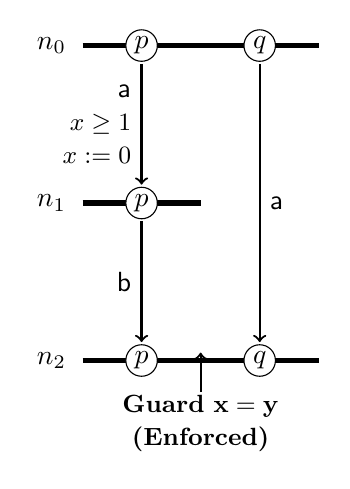
\begin{tikzpicture}
    % Nodes (Bars)
    \draw[line width=2pt] (0,4) node[left] {$n_0\,$} -- (3,4);
    \draw[line width=2pt] (0,2) node[left] {$n_1\,$} -- (1.5,2);
    \draw[line width=2pt] (0,0) node[left] {$n_2\,$} -- (3,0);

    % Ports
    \filldraw[fill=white] (0.75,4) circle (2mm) node (p_n0) {$p$};
    \filldraw[fill=white] (2.25,4) circle (2mm) node (q_n0) {$q$};
    
    \filldraw[fill=white] (0.75,2) circle (2mm) node (p_n1) {$p$};
    
    \filldraw[fill=white] (0.75,0) circle (2mm) node (p_n2) {$p$};
    \filldraw[fill=white] (2.25,0) circle (2mm) node (q_n2) {$q$};

    % Edges
    % p: n0 -> n1
    \draw[->, thick] (p_n0) -- (p_n1) node[midway, left, align=right] {$\mathsf{a}$ \\ \small $x \ge 1$ \\ \small $x:=0$};
    
    % q: n0 -> n2
    \draw[->, thick] (q_n0) -- (q_n2) node[midway, right] {$\mathsf{a}$};

    % p: n1 -> n2
    \draw[->, thick] (p_n1) -- (p_n2) node[midway, left] {$\mathsf{b}$};

    % Guard visualization
    \node[align=center] at (1.5, -0.8) {\small \textbf{Guard} $\mathbf{x=y}$ \\ \small \textbf{(Enforced)}};
    \draw[->, thick] (1.5, -0.4) -- (1.5, 0.1);
\end{tikzpicture}
}
\caption{\textbf{Always-Synchronizing.} Every node acts as a synchronization barrier. The execution behaves like a global-time system. The guard $x=y$ is strictly enforced, requiring $p$ and $q$ to reach $n_2$ with equal clock values.}
\label{fig:ltn_always_sync}
\end{subfigure}

\caption{The running example LTN interpreted under two different semantic assumptions. Structurally they are identical, but the role of the guard at $n_2$ differs.}
\label{fig:running_example_comparison}
\end{figure}

We will interpret this negotiation~\ref{fig:running_example_comparison} under different synchronization
assumptions:
\begin{itemize}
\item In synchronization-free LTNs, $n_2$ does not enforce equality of
reference clocks, and the comparison $x = y$ becomes ineffective.
\item In always-synchronizing LTNs, every node enforces synchronization
so the entire execution admits a global-time interpretation.
\item In general LTNs, the combination of unsynchronized drift at $n_1$
and synchronization at $n_2$ enables comparison of accumulated delays,
which underlies undecidability.
\end{itemize}

\paragraph{Why the extremes avoid undecidability.}
The running example above also illustrates why undecidability requires
\emph{selective} synchronization.

Suppose $n_1$ is unsynchronized while $n_2$ is synchronizing.
Agent $p$ may delay arbitrarily at $n_1$, increasing its reference clock
$t_p$, while agent $q$ does not participate and its reference clock
remains unchanged.
At the synchronizing node $n_2$, the equality constraint $t_p = t_q$
forces agent $q$ to ``catch up'', effectively testing how much delay
$p$ accumulated earlier.

This pattern—unbounded drift at unsynchronized nodes followed by
comparison at synchronized nodes—allows encoding and testing unbounded
counters.
It is precisely this interaction that is excluded in the two extremes:
\begin{itemize}
\item In synchronization-free LTNs, there is no point at which drift can
  be tested.
\item In always-synchronizing LTNs, drift cannot accumulate between
  interactions.
\end{itemize}

General LTNs permit both behaviors simultaneously, leading to
undecidability.
\end{comment}
%%%%%%%%%%%%%%%%%%%%%%%%%%%%%%%%%%%%%%%%%%%%%%%%%%%
%---------------------------------------------------------------------------------

\section{Synchronization-Free LTNs}
\label{sec:syncfree}

\subsection{Definition and Behavior}

\begin{definition}[Synchronization-free LTN]
\label{def:syncfree}
An LTN $\mathcal{N} = (N, \text{dom}, \delta, \text{Sync})$ is \textsf{synchronization-free} if $\text{Sync} = \emptyset$.
\end{definition}

In synchronization-free LTNs, no action step requires equality of reference clocks. When location $(n, a)$ is executed, participating agents must satisfy their local guards (constraints on clocks in $X_p$), but their reference clocks $t_p$ need not be equal. Agents accumulate local time independently between interactions, coordinating only through control flow (markings) and timing constraints (guards), never through explicit temporal alignment.

\paragraph{Expressiveness implications.} Recall the examples from Chapter~\ref{chap:ltn}:

\begin{itemize}
\item \textbf{Vendor example (Figure~\ref{fig:vendor})}: If $n_3$ is not synchronizing, agent $q$ need not visit the vendor to "catch up" to $p$'s reference clock. The causal enforcement mechanism disappears—$q$ can proceed directly from $n_1$ to $n_3$ as soon as control flow permits and guards are satisfied.

\item \textbf{$a^n b^n c^n$ example (Figure~\ref{fig:abc})}: If $n_3$ is not synchronizing, the language changes dramatically. Without synchronization forcing $t_p = t_q$, there's no mechanism to compare how many $a$'s versus $b$'s occurred. The untimed language becomes simply $\{w \cdot c \mid w \in \{a, b\}^*, \, w \text{ contains} \geq 1 \, a \text{ and} \geq 1 \, b\}$ (any interleaving with at least one of each), which is regular.
\end{itemize}

Since $\text{Sync} = \emptyset$, no action step tests $t_p = t_q$, and reference clocks $t_p$ never appear in any guard and are never reset (by definition, guards use only clocks in $X_p$), only advance monotonically. Therefore, for reachability purposes, the absolute values of reference clocks are irrelevant—only the values of local clocks in $X$ matter. 

The following example illustrates that although each agent's timing constraints are local, the combination of guards across agents at a location can create implicit coordination requirements. Consider Figure~\ref{fig:coord}:

\begin{figure}[htb]
\centering 
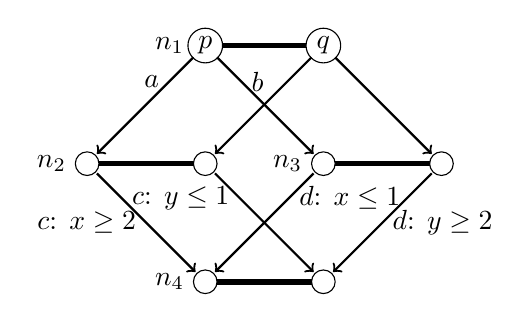
\begin{tikzpicture}[scale=1, every node/.style={transform shape}]

\begin{scope}[line width=2pt]
\draw (0,0) node [left] {$n_1\,\,$} -- (1.5,0);
\draw (-1.5,-1.5) node [left] {$n_2\,\,$} -- (0,-1.5);
\draw (1.5,-1.5) node [left] {$n_3\,\,$} -- (3,-1.5);
\draw (0,-3) node [left] {$n_4\,\,$} -- (1.5,-3);
\end{scope}

\filldraw [fill=white]  (0,0)  circle (2.2mm) node (n1p) {$p$};
\filldraw [fill=white]  (1.5,0)  circle (2.2mm) node (n1q) {$q$};

\filldraw [fill=white]  (-1.5,-1.5)  circle (1.5mm) node (n2p) {};
\filldraw [fill=white]  (0,-1.5)  circle (1.5mm) node (n2q) {};

\filldraw [fill=white]  (1.5,-1.5)  circle (1.5mm) node (n3p) {};
\filldraw [fill=white]  (3,-1.5)  circle (1.5mm) node (n3q) {};

\filldraw [fill=white]  (0,-3)  circle (1.5mm) node (n4p) {};
\filldraw [fill=white]  (1.5,-3)  circle (1.5mm) node (n4q) {};

\begin{scope}[thick,->]
\draw (n1p) + (-0.15,-0.15) -- (n2p) node [near start, left] {$a$};
\draw (n1q) + (-0.15,-0.15) -- (n2q);

\draw (n1p) + (0.15,-0.15) -- (n3p) node [near start, right] {$b$};
\draw (n1q) + (0.15,-0.15) -- (n3q);

\draw (n2p) -- (n4p) node [midway, left] {$c$: $x \geq 2$};
\draw (n2q) -- (n4q) node [near start, left] {$c$: $y \leq 1$};

\draw (n3p) -- (n4p) node [near start, right] {$d$: $x \leq 1$};
\draw (n3q) -- (n4q) node [midway, right] {$d$: $y \geq 2$};
\end{scope}

\end{tikzpicture}
\caption{Synchronization-free LTN illustrating implicit coordination. At $n_1$, agents $p$ and $q$ non-deterministically choose outcome $a$ or $b$. For outcome $c$ at $n_4$ to be feasible, both must have chosen $a$ (route through $n_2$), since $c$ requires $x \geq 2$ from $p$ and $y \leq 1$ from $q$—constraints incompatible with the $b$-route guards.}
\label{fig:coord}
\end{figure}

At $n_1$, outcome $a$ or $b$ is chosen non-deterministically. To reach location $(n_4, c)$, both agents must route through $n_2$ (both choosing $a$), since $c$ requires $x \geq 2$ from $p$ and $y \leq 1$ from $q$. Routing through $n_3$ (via outcome $b$) imposes $x \leq 1$ for $p$ and $y \geq 2$ for $q$. These constraints make $(n_4, c)$ unreachable if either agent chose $b$. Thus, local timing decisions at $n_1$ have global reachability consequences, even without explicit synchronization. The agents must implicitly `agree' on a path to make later locations feasible.

\subsection{Product-region abstraction}
\paragraph{Geometric intuition.}
In synchronization-free LTNs, each agent evolves according to its own
local clocks without ever comparing time with other agents.
Consequently, the global time state of the system can be seen as a tuple
of independent local time states—one per agent.

For each agent $p$, the standard region abstraction partitions
$\mathbb{R}_{\ge 0}^{X_p}$ into finitely many regions.
The global abstraction is then obtained by taking the Cartesian product
of these per-agent partitions.
Two global valuations are equivalent if and only if they are equivalent
for each agent separately.

Intuitively, synchronization-free LTNs behave like a collection of
independent timed automata whose discrete transitions must occur
together at negotiation nodes, but whose timing evolution is otherwise
decoupled.

Let
\[
  M := \max\{\,c \mid \text{$c$ appears in some atomic constraint $x\bowtie c$ of a guard in $\Nn$}\,\}.
\]
In this fragment, reference clocks $T=\{t_p\mid p\in P\}$ do not appear in guards
and are never tested for synchronization. Thus, for reachability, it suffices to
abstract only the local clocks $X$.

We define a region equivalence \emph{per agent} and take their product.

\begin{definition}[Per-agent region equivalence]
\label{def:per-agent-region}
Fix an agent $p \in P$. For valuations $v, v' : X_p \to \mathbb{R}_{\geq 0}$, write $v \sim^p_M v'$ if for all clocks $x, y \in X_p$:
\begin{enumerate}
\item \textbf{Integer parts agree (or both exceed $M$):} \\
Either $\lfloor v(x) \rfloor = \lfloor v'(x) \rfloor$, or both $\lfloor v(x) \rfloor > M$ and $\lfloor v'(x) \rfloor > M$.

\item \textbf{Zero fractional parts agree:} \\
If $v(x) \leq M$, then $\text{frac}(v(x)) = 0$ iff $\text{frac}(v'(x)) = 0$.

\item \textbf{Fractional orderings agree (for clocks $\leq M$):} \\
If $v(x) \leq M$ and $v(y) \leq M$, then $\text{frac}(v(x)) \leq \text{frac}(v(y))$ iff $\text{frac}(v'(x)) \leq \text{frac}(v'(y))$.
\end{enumerate}
\end{definition}

This is precisely the standard timed-automata region equivalence~\cite{DBLP:journals/tcs/AlurD94} applied to clocks $X_p$ of agent $p$.

\begin{definition}[Product-region equivalence]
\label{def:product-region}
For valuations $v, v' : X \to \mathbb{R}_{\geq 0}$ (over all local clocks), write $v \sim_{\text{pr}} v'$ if:
\[
v|_{X_p} \sim^p_M v'|_{X_p} \quad \text{for every agent } p \in P.
\]
We call $\sim_{\text{pr}}$ the \emph{product-region equivalence}. Let $[v]_{\text{pr}}$ denote the equivalence class of $v$.
\end{definition}

\begin{lemma}[Finite index]
\label{lem:size-of-product-regions}
The product-region equivalence $\sim_{\mathrm{pr}}$ has finite index. In
particular, the number of product-regions is bounded by
$\Oo(|X|!\cdot 2^{|X|}\cdot (2M+2)^{|X|})$.
\end{lemma}

%========================
% Lemma 5.3 (Finite index)
%========================
\begin{proof}[Proof of Lemma~\ref{lem:size-of-product-regions}]
Fix an agent $p\in P$ and let $k_p := |X_p|$.  We first bound the number of
$\sim^p_M$-classes over valuations of $X_p$, and then take the product over all
agents.

A $\sim^p_M$-class is determined by the following finite data:

\medskip\noindent
\textbf{(A) Truncated integer parts.}
For each $x\in X_p$, define its \emph{truncated integer part}
\[
  \iota(x) \;:=\;
  \begin{cases}
    \lfloor v(x)\rfloor & \text{if } \lfloor v(x)\rfloor \le M,\\
    M+1 & \text{if } \lfloor v(x)\rfloor > M.
  \end{cases}
\]
Thus $\iota(x)\in\{0,1,\dots,M,M+1\}$, giving at most $(M+2)^{k_p}$ possibilities.

\medskip\noindent
\textbf{(B) Zero/nonzero fractional flags for clocks not above $M$.}
For each $x\in X_p$ with $\iota(x)\le M$ we record the Boolean
\[
  z(x) \;:=\; \bigl( \{v(x)\}=0 \bigr).
\]
For clocks with $\iota(x)=M+1$ (i.e.\ $v(x)>M$) this flag is irrelevant in the
definition of $\sim^p_M$, so we may still count it pessimistically. This yields
at most $2^{k_p}$ possibilities.

\medskip\noindent
\textbf{(C) Ordering of fractional parts among clocks not above $M$.}
Let $S := \{x\in X_p \mid \iota(x)\le M\}$.
The third bullet in Definition~\ref{def:product-region} requires that for all
$x,y\in S$,
\[
  \{v(x)\}\le \{v(y)\} \quad\text{iff}\quad \{v'(x)\}\le \{v'(y)\}.
\]
Equivalently, it fixes the total preorder of the multiset
$\bigl(\{v(x)\}\bigr)_{x\in S}$.
Any total preorder on $|S|\le k_p$ elements can be obtained by taking a total
order and allowing ties; hence the number of such preorders is bounded by
$k_p!\cdot 2^{k_p}$ (choose an order, then choose where to merge adjacent items).
Therefore, the number of possibilities for (C) is at most $k_p!\cdot 2^{k_p}$.

\medskip
Combining (A), (B), (C), the number of $\sim^p_M$-classes is bounded by
\[
  (M+2)^{k_p}\cdot 2^{k_p}\cdot (k_p!\cdot 2^{k_p})
  \;=\; k_p!\cdot 2^{2k_p}\cdot (M+2)^{k_p}.
\]

Now $\sim_{\mathrm{pr}}$ is the product of the per-agent relations, so the number
of product-regions is at most the product over agents:
\[
  \prod_{p\in P} \Bigl(k_p!\cdot 2^{2k_p}\cdot (M+2)^{k_p}\Bigr)
  \;=\;
  \Bigl(\prod_{p} k_p!\Bigr)\cdot 2^{2\sum_p k_p}\cdot (M+2)^{\sum_p k_p}.
\]
Since $\sum_p k_p = |X|$ and $\prod_p k_p! \le |X|!$, we obtain
\[
  \#\text{(product-regions)} \;\le\; |X|!\cdot 2^{2|X|}\cdot (M+2)^{|X|}.
\]
Finally, using $M+2 \le 2M+2$ for $M\ge 0$ and absorbing the extra $2^{|X|}$ into
the $\mathcal{O}$-notation, we get the stated bound
\[
  \#\text{(product-regions)} \;=\; \mathcal{O}\bigl(|X|!\cdot 2^{|X|}\cdot (2M+2)^{|X|}\bigr).
\]
Hence $\sim_{\mathrm{pr}}$ has finite index.
\end{proof}

\begin{lemma}[Compatibility with local delays]
\label{lemma:region-local-delay}
Let $v \sim_{\mathrm{pr}} v'$. For every local delay vector $\Delta\in \Rpos^{P}$
there exists a local delay vector $\Delta'$ such that
$v+\Delta \sim_{\mathrm{pr}} v'+\Delta'$.
\end{lemma}

%\begin{proof}[Proof sketch]
%The claim follows componentwise from the standard time-elapse property of region equivalence for timed automata (Chapter~\ref{chap:preliminaries}): for each agent $p$, from $v|_{X_p}\sim^p_M v'|_{X_p}$ and the delay $\Delta(p)$ we obtain some $\Delta'(p)$ such that $v|_{X_p}+\Delta(p) \sim^p_M v'|_{X_p}+\Delta'(p)$. Taking the product over all agents yields the stated $\Delta'$.
%\end{proof}

%=========================================
% Lemma 5.4 (Compatibility with local delays)
%=========================================
\begin{proof}
Assume $v \sim_{\mathrm{pr}} v'$ and fix a local delay vector
$\Delta\in\Rpos^{P}$.
We construct a local delay vector $\Delta'\in\Rpos^{P}$ such that
$v+\Delta \sim_{\mathrm{pr}} v'+\Delta'$.

Fix an agent $p\in P$ and write $v_p := v|_{X_p}$ and $v'_p := v'|_{X_p}$.
By definition of $\sim_{\mathrm{pr}}$, we have $v_p \sim^p_M v'_p$.

Now consider the standard timed-automata region equivalence on the clock set
$X_p$ with maximal constant $M$; our relation $\sim^p_M$ is exactly this
equivalence (restricted to clocks of agent $p$).
By the time-elapse compatibility of regions proved in the preliminaries
(Lemma~\ref{lem:TA-region-time-elapse}), from $v_p \sim^p_M v'_p$ and
$d:=\Delta(p)\ge 0$ we obtain a delay $d'\ge 0$ such that
\[
  v_p + d \;\sim^p_M\; v'_p + d'.
\]
Define $\Delta'(p):=d'$.

Doing this independently for every agent $p$ yields a vector
$\Delta'\in \Rpos^{P}$ satisfying, for each $p$,
\[
  (v+\Delta)|_{X_p} \;=\; v_p+\Delta(p) \;\sim^p_M\; v'_p+\Delta'(p)
  \;=\; (v'+\Delta')|_{X_p}.
\]
Since $\sim_{\mathrm{pr}}$ is defined componentwise over agents, this implies
$v+\Delta \sim_{\mathrm{pr}} v'+\Delta'$, as required.
\end{proof}

\begin{lemma}[Compatibility with guards and resets]
\label{lem:region-guard-reset}
Let $v \sim_{\mathrm{pr}} v'$. Let $g$ be any guard whose constants are at most
$M$. Then:
\begin{enumerate}
  \item $v\models g$ iff $v'\models g$;
  \item for every set of local clocks $Y\subseteq X$, we have $v[Y]\sim_{\mathrm{pr}} v'[Y]$.
\end{enumerate}
\end{lemma}

%=========================================
% Lemma 5.5 (Compatibility with guards and resets)
%=========================================
\begin{proof}
Assume $v \sim_{\mathrm{pr}} v'$, and let $g$ be any guard whose constants are at
most $M$. By the syntax used in the chapter, $g$ is a Boolean combination of
atomic constraints of the form $x \bowtie c$ where $c\in\{0,1,\dots,M\}$ and
$\bowtie\in\{<,\le,=,\ge,>\}$, and $x$ is a local clock.

\medskip\noindent
\textbf{(1) Preservation of guard satisfaction.}
Since $g$ is a Boolean combination, it suffices to prove preservation for a
single atomic constraint $x\bowtie c$.

Fix such an atom. Let $p$ be the unique agent with $x\in X_p$.
From $v \sim_{\mathrm{pr}} v'$ we get $v|_{X_p} \sim^p_M v'|_{X_p}$, hence in
particular:
\begin{itemize}
  \item either $\lfloor v(x)\rfloor=\lfloor v'(x)\rfloor$, or both
        $\lfloor v(x)\rfloor > M$ and $\lfloor v'(x)\rfloor > M$;
  \item if $v(x)\le M$ then $\{v(x)\}=0$ iff $\{v'(x)\}=0$.
\end{itemize}

Now consider cases.

\smallskip\noindent
\emph{Case I: $v(x)>M$.}
Then $v'(x)>M$ as well. Since $c\le M$, we have $v(x)\bowtie c$ iff $v'(x)\bowtie c$
for all $\bowtie\in\{>,\ge\}$ (both true) and for all $\bowtie\in\{<,\le,=\}$
(both false). So the atom is preserved.

\smallskip\noindent
\emph{Case II: $v(x)\le M$.}
Then $\lfloor v(x)\rfloor=\lfloor v'(x)\rfloor=:k\le M$.
Write $v(x)=k+f$ and $v'(x)=k+f'$ with $f,f'\in[0,1)$ and $f=0$ iff $f'=0$.

Because $c$ is an integer, the truth of $x\bowtie c$ depends only on:
(i) whether $k<c$, $k>c$, or $k=c$; and (ii) in the boundary case $k=c$, whether
the fractional part is $0$ or not.

Indeed:
\begin{itemize}
  \item $v(x) < c$ iff $k<c$;
  \item $v(x) \le c$ iff $k<c$ or ($k=c$ and $f=0$);
  \item $v(x) = c$ iff $k=c$ and $f=0$;
  \item $v(x) \ge c$ iff $k>c$ or ($k=c$ and $f=0$);
  \item $v(x) > c$ iff $k>c$.
\end{itemize}
All these conditions are preserved when replacing $(k,f)$ by $(k,f')$ because
$k$ is the same and $f=0 \Leftrightarrow f'=0$.
Hence $v\models (x\bowtie c)$ iff $v'\models (x\bowtie c)$.

This proves preservation for atoms, hence for any Boolean combination $g$.

\medskip\noindent
\textbf{(2) Preservation under resets.}
Let $Y\subseteq X$ be any set of local clocks to reset to $0$.
We must show $v[Y]\sim_{\mathrm{pr}} v'[Y]$.

Fix an agent $p$. We show $(v[Y])|_{X_p} \sim^p_M (v'[Y])|_{X_p}$.
Let $Y_p := Y\cap X_p$. Then $(v[Y])|_{X_p}$ is obtained from $v|_{X_p}$ by
setting clocks in $Y_p$ to $0$ (and leaving others unchanged), and similarly for
$v'$.

Take any $x\in X_p$.
\begin{itemize}
  \item If $x\in Y_p$, then both valuations assign $0$ to $x$, so the first two
        bullets of $\sim^p_M$ hold trivially for $x$.
  \item If $x\notin Y_p$, then $v[Y](x)=v(x)$ and $v'[Y](x)=v'(x)$, so the first
        two bullets hold because they held for $v$ and $v'$.
\end{itemize}
For the third bullet (ordering of fractional parts among clocks $\le M$), note
that every reset clock has fractional part $0$, and every non-reset clock keeps
its old fractional part. Since in $v$ and $v'$ the relative order relations
$\{v(x)\}\le \{v(y)\}$ among clocks $\le M$ were identical, and since we apply
the same transformation “set some designated clocks to $0$” on both sides, the
resulting order relations among fractional parts remain identical as well.
Formally, for any $x,y\in X_p$ with $(v[Y])(x)\le M$ and $(v[Y])(y)\le M$:
\begin{itemize}
  \item if both are not reset, the relation is the same as before;
  \item if one is reset, its fractional part becomes $0$ on both sides;
  \item if both are reset, both fractional parts are $0$ on both sides.
\end{itemize}
Hence the iff-condition in the third bullet is preserved.

Therefore $(v[Y])|_{X_p}\sim^p_M (v'[Y])|_{X_p}$ for every $p$, i.e.\
$v[Y]\sim_{\mathrm{pr}} v'[Y]$.
\end{proof}

\subsection{The product-region automaton}

We now build a finite automaton over locations that captures precisely the
feasible untimed location sequences of a synchronization-free LTN.

\begin{definition}[Product-region automaton]
\label{def:pr-automaton}
Let $\mathcal{N}$ be synchronization-free. The \textsf{product-region automaton} $\mathcal{A}_{\text{pr}}(\mathcal{N})$ is an NFA with:
\begin{itemize}
\item \textbf{States}: pairs $(C, r)$ where $C$ is a marking and $r$ is a product-region.

\item \textbf{Transitions}: $(C, r) \xrightarrow{(n,a)} (C', r')$ iff there exist $v \in r$ and local delay $\Delta$ such that:
\[
(C, v) \xrightarrow{\Delta} (C, v + \Delta) \xrightarrow{(n,a)} (C', v')
\]
in $\mathcal{N}$, with $v' \in r'$.

\item \textbf{Initial state}: $(C_0, [v_0]_{\text{pr}})$ where $C_0(p) = \{n_{\text{in}}\}$ for all $p$, and $v_0$ maps all clocks in $X$ to 0.
\end{itemize}
\end{definition}

% ------------------------------------------------------------------
% Explicit product-region calculations for the running (sync-free) example
% (adapted to satisfy the "guards are local" assumption in this chapter)
% ------------------------------------------------------------------

\subsection{Product-Region Calculations on an Example}
\label{subsec:explicit-pr-example}

We illustrate the product-region abstraction (Section~\ref{sec:syncfree}) by
working out regions explicitly on a tiny synchronization-free LTN instance.
Recall that in our model, each agent's guard mentions only its own local clocks
(see Lemma~\ref{lem:product-region-compat}(2)).\,\footnote{This locality
assumption is used throughout this chapter.}

\paragraph{The example.}
Let $P=\{p,q\}$, with local clocks $X_p=\{x\}$ and $X_q=\{y\}$.
Consider three nodes $N=\{n_0,n_1,n_2\}$ with
\[
\dom(n_0)=\{p,q\},\qquad \dom(n_1)=\{p\},\qquad \dom(n_2)=\{p,q\}.
\]
We fix outcomes $a,b,c$ and local transition data:
\begin{itemize}
\item At $(n_0,a)$: no guards, no resets (only control-flow updates).
\item At $(n_1,b)$ (agent $p$ only): guard $x \ge 1$, reset $x:=0$.
\item At $(n_2,c)$ (agents $p,q$): for $q$ we require guard $y \ge 1$ and reset $y:=0$
      (agent $p$ has trivial guard/reset at this step).
\end{itemize}
This example is synchronization-free, i.e.\ $\Sync=\emptyset$.

\begin{figure}[htb]
\centering 
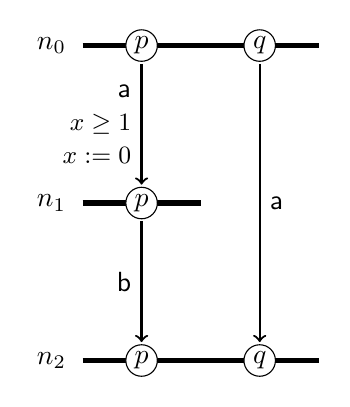
\begin{tikzpicture}[scale=1, every node/.style={transform shape}]

    % Nodes (Bars)
    \draw[line width=2pt] (0,4) node[left] {$n_0\,$} -- (3,4);
    \draw[line width=2pt] (0,2) node[left] {$n_1\,$} -- (1.5,2);
    \draw[line width=2pt] (0,0) node[left] {$n_2\,$} -- (3,0);

    % Ports
    \filldraw[fill=white] (0.75,4) circle (2mm) node (p_n0) {$p$};
    \filldraw[fill=white] (2.25,4) circle (2mm) node (q_n0) {$q$};
    
    \filldraw[fill=white] (0.75,2) circle (2mm) node (p_n1) {$p$};
    
    \filldraw[fill=white] (0.75,0) circle (2mm) node (p_n2) {$p$};
    \filldraw[fill=white] (2.25,0) circle (2mm) node (q_n2) {$q$};

    % Edges
    % p: n0 -> n1
    \draw[->, thick] (p_n0) -- (p_n1) node[midway, left, align=right] {$\mathsf{a}$ \\ \small $x \ge 1$ \\ \small $x:=0$};
    
    % q: n0 -> n2 (Wait)
    \draw[->, thick] (q_n0) -- (q_n2) node[midway, right] {$\mathsf{a}$};

    % p: n1 -> n2
    \draw[->, thick] (p_n1) -- (p_n2) node[midway, left] {$\mathsf{b}$};

\end{tikzpicture}
\caption{A simple synchronization-free LTN.}
\label{fig:coord}
\end{figure}

\paragraph{Maximal constant.}
The only constants appearing in guards are $1$, hence
\[
M = 1.
\]

\subsubsection*{Per-agent regions for one clock (with $M=1$)}
Since each agent has a single clock, the standard region
equivalence partitions $\mathbb{R}_{\ge 0}$ into four regions:
\begin{align*}
R^0 &:= \{z \mid z = 0\},\\
R^{(0,1)} &:= \{z \mid 0 < z < 1\},\\
R^{1} &:= \{z \mid z = 1\},\\
R^{>1} &:= \{z \mid z > 1\}.
\end{align*}
For agent $p$ (clock $x$) we write these as $R_x^0, R_x^{(0,1)}, R_x^{1}, R_x^{>1}$,
and similarly for agent $q$ (clock $y$) we write $R_y^0, R_y^{(0,1)}, R_y^{1}, R_y^{>1}$.

\subsubsection*{Product regions}
A product-region is a pair of per-agent regions:
\[
r \;=\; R_x^{\alpha}\times R_y^{\beta}
\qquad\text{where}\qquad
\alpha,\beta \in \{0,(0,1),1,>1\}.
\]
Hence there are $4\cdot 4 = 16$ product-regions in total.

\paragraph{Guard satisfaction at the region level.}
With $M=1$ and one clock per agent:
\[
x \ge 1 \text{ holds exactly on } R_x^1 \cup R_x^{>1},
\qquad
y \ge 1 \text{ holds exactly on } R_y^1 \cup R_y^{>1}.
\]
This is the concrete instantiation of Lemma~\ref{lem:product-region-compat}(2).

\subsubsection*{A concrete run and its product-region trace}
We now pick explicit local delays (a delay vector $\Delta\in\mathbb{R}_{\ge 0}^P$)
and track the induced product-region sequence.

\paragraph{Initial valuation.}
Let $v_0(x)=0$ and $v_0(y)=0$. Then
\[
(x,y)=(0,0)\in R_x^0\times R_y^0,
\quad\text{so}\quad
r_0 := [v_0]_{pr} = R_x^0\times R_y^0.
\]

\paragraph{Step 1: delay then $(n_1,b)$.}
Choose a local delay $\Delta_0$ with
\[
\Delta_0(p)=1.3,\qquad \Delta_0(q)=0.4.
\]
After delay, we have
\[
(x,y)=(1.3,0.4)\in R_x^{>1}\times R_y^{(0,1)},
\quad\text{so}\quad
r_1 = R_x^{>1}\times R_y^{(0,1)}.
\]
Now $(n_1,b)$ is enabled because $x\ge 1$ holds in $R_x^{>1}$.
Executing $(n_1,b)$ resets $x:=0$, yielding
\[
(x,y)=(0,0.4)\in R_x^0\times R_y^{(0,1)},
\quad\text{so}\quad
r_2 = R_x^0\times R_y^{(0,1)}.
\]

\paragraph{Step 2: delay then $(n_2,c)$.}
Choose a local delay $\Delta_1$ with
\[
\Delta_1(p)=0.2,\qquad \Delta_1(q)=0.8.
\]
After delay, we have
\[
(x,y)=(0.2,1.2)\in R_x^{(0,1)}\times R_y^{>1},
\quad\text{so}\quad
r_3 = R_x^{(0,1)}\times R_y^{>1}.
\]
Now $(n_2,c)$ is enabled because $y\ge 1$ holds in $R_y^{>1}$.
Executing $(n_2,c)$ resets $y:=0$, yielding
\[
(x,y)=(0.2,0)\in R_x^{(0,1)}\times R_y^0,
\quad\text{so}\quad
r_4 = R_x^{(0,1)}\times R_y^{0}.
\]

\paragraph{Region-trace summary.}
Altogether, this concrete run induces the product-region trace
\[
R_x^0\times R_y^0
\;\xrightarrow{\Delta_0=(1.3,\,0.4)}\;
R_x^{>1}\times R_y^{(0,1)}
\;\xrightarrow{(n_1,b):\,x\ge 1,\ x:=0}\;
R_x^{0}\times R_y^{(0,1)}
\;\xrightarrow{\Delta_1=(0.2,\,0.8)}\;
R_x^{(0,1)}\times R_y^{>1}
\;\xrightarrow{(n_2,c):\,y\ge 1,\ y:=0}\;
R_x^{(0,1)}\times R_y^{0}.
\]
This makes the product abstraction fully explicit: the global abstract state
changes by (i) componentwise time-elapse within each per-agent region partition,
followed by (ii) componentwise resets triggered by discrete steps.

\begin{lemma}[Soundness and completeness]
\label{lem:reg-prod-reg-equiv}
Assume $\Nn$ is synchronization-free.
\begin{enumerate}
  \item For every run of $\Nn$
  \[
  (C_0,v_0)\xra{\Delta_0,(n_0,a_0)}(C_1,v_1)\xra{\Delta_1,(n_1,a_1)}\cdots\xra{\Delta_{m-1},(n_{m-1},a_{m-1})}(C_m,v_m),
  \]
  there exists a run in $\prg(\Nn)$
  \[
  (C_0,\region{v_0})\xra{(n_0,a_0)}(C_1,\region{v_1})\xra{(n_1,a_1)}\cdots\xra{(n_{m-1},a_{m-1})}(C_m,\region{v_m}).
  \]
  \item Conversely, for every run in $\prg(\Nn)$
  \[
  (C_0,r_0)\xra{(n_0,a_0)}(C_1,r_1)\xra{(n_1,a_1)}\cdots\xra{(n_{m-1},a_{m-1})}(C_m,r_m),
  \]
  there exists a run in $\Nn$
  \[
  (C_0,v_0)\xra{\Delta_0,(n_0,a_0)}(C_1,v_1)\xra{\Delta_1,(n_1,a_1)}\cdots\xra{\Delta_{m-1},(n_{m-1},a_{m-1})}(C_m,v_m)
  \]
  such that $v_i\in r_i$ for all $0\le i\le m$.
\end{enumerate}
\end{lemma}

%=========================================
% Lemma 5.7 (Soundness and completeness)
%=========================================
\begin{proof}[Detailed proof of Lemma~\ref{lem:reg-prod-reg-equiv}]
Assume $\Nn$ is synchronization-free, so only local clocks $X$ matter and there
is no synchronization test involving reference clocks.

\medskip\noindent
\textbf{(1) Soundness (from $\Nn$ to $\prg(\Nn)$).}
Let
\[
(C_0,v_0)\xra{\Delta_0,(n_0,a_0)}(C_1,v_1)\xra{\Delta_1,(n_1,a_1)}\cdots
\xra{\Delta_{m-1},(n_{m-1},a_{m-1})}(C_m,v_m)
\]
be a run of $\Nn$.
By the LTN semantics, each macro-step
$\xra{\Delta_i,(n_i,a_i)}$ abbreviates a small-step decomposition
\[
(C_i,v_i)\xra{\Delta_i}(C_i,v_i+\Delta_i)\xra{(n_i,a_i)}(C_{i+1},v_{i+1}).
\]
Set $r_i:=\region{v_i}$ for each $i$.
By Definition~\ref{def:prod-reg-aut} of $\prg(\Nn)$, a transition
\[
(C_i,r_i)\xra{(n_i,a_i)}(C_{i+1},r_{i+1})
\]
exists whenever there are witnesses $v\in r_i$, $\Delta\ge 0$ such that
$(C_i,v)\xra{\Delta}(C_i,v+\Delta)\xra{(n_i,a_i)}(C_{i+1},v')$ with $v'\in r_{i+1}$.
We can take the concrete witnesses $v:=v_i$, $\Delta:=\Delta_i$, and $v':=v_{i+1}$.
Thus every step of the $\Nn$-run induces a corresponding step in $\prg(\Nn)$,
yielding the run
\[
(C_0,\region{v_0})\xra{(n_0,a_0)}(C_1,\region{v_1})\xra{(n_1,a_1)}\cdots
\xra{(n_{m-1},a_{m-1})}(C_m,\region{v_m}).
\]

\medskip\noindent
\textbf{(2) Completeness (from $\prg(\Nn)$ to $\Nn$).}
Let
\[
(C_0,r_0)\xra{(n_0,a_0)}(C_1,r_1)\xra{(n_1,a_1)}\cdots
\xra{(n_{m-1},a_{m-1})}(C_m,r_m)
\]
be a run of $\prg(\Nn)$.
We construct, by induction on $i=0,\dots,m$, valuations $v_i\in r_i$ and local
delays $\Delta_i$ (for $i<m$) such that
\[
(C_i,v_i)\xra{\Delta_i}(C_i,v_i+\Delta_i)\xra{(n_i,a_i)}(C_{i+1},v_{i+1})
\]
is a valid small-step decomposition in $\Nn$.

\smallskip\noindent
\emph{Base $i=0$.}
By construction of $\prg(\Nn)$, $r_0=\region{v_0}$ where $v_0$ is the all-zero
valuation, so choose $v_0$ accordingly.

\smallskip\noindent
\emph{Induction step.}
Assume $v_i\in r_i$ has been chosen.
Consider the automaton transition
\[
(C_i,r_i)\xra{(n_i,a_i)}(C_{i+1},r_{i+1}).
\]
By Definition~\ref{def:prod-reg-aut}, there exist witnesses:
a valuation $u_i\in r_i$, a local delay vector $\widehat{\Delta}_i$, and a
valuation $u_{i+1}\in r_{i+1}$ such that in $\Nn$,
\[
(C_i,u_i)\xra{\widehat{\Delta}_i}(C_i,u_i+\widehat{\Delta}_i)\xra{(n_i,a_i)}(C_{i+1},u_{i+1})
\]
is a valid pair of steps.

Now $v_i\in r_i$ and $u_i\in r_i$ imply $v_i \sim_{\mathrm{pr}} u_i$.
Apply Lemma~\ref{lemma:region-local-delay} to $v_i \sim_{\mathrm{pr}} u_i$ and
delay $\widehat{\Delta}_i$ to obtain a (possibly different) local delay vector
$\Delta_i$ such that
\[
v_i+\Delta_i \;\sim_{\mathrm{pr}}\; u_i+\widehat{\Delta}_i. \tag{$\ast$}
\]
We claim that $(n_i,a_i)$ is enabled from $(C_i, v_i+\Delta_i)$ and that firing it
produces some $v_{i+1}\in r_{i+1}$.

Let $g$ be the conjunction of all local guards required for executing outcome
$(n_i,a_i)$ (one per participating agent, combined as in the LTN semantics).
Since $\Nn$ is synchronization-free, $g$ depends only on local clocks and uses
only constants $\le M$ (by definition of $M$ in the chapter).
Because $u_i+\widehat{\Delta}_i$ enables $(n_i,a_i)$, we have
$u_i+\widehat{\Delta}_i \models g$.
By ($\ast$) and Lemma~\ref{lem:region-guard-reset}(1), we also have
$v_i+\Delta_i \models g$, hence $(n_i,a_i)$ is enabled from $(C_i,v_i+\Delta_i)$.

Let $Y\subseteq X$ be the set of local clocks reset by firing $(n_i,a_i)$
(across all agents in $\dom(n_i)$, exactly as prescribed by $\delta$).
In a synchronization-free LTN, the discrete step sets precisely those clocks in
$Y$ to $0$ and leaves the others unchanged; thus the successor valuation is
\[
v_{i+1} := (v_i+\Delta_i)[Y], \qquad
u_{i+1} := (u_i+\widehat{\Delta}_i)[Y].
\]
By Lemma~\ref{lem:region-guard-reset}(2) applied to ($\ast$), we get
\[
(v_i+\Delta_i)[Y] \;\sim_{\mathrm{pr}}\; (u_i+\widehat{\Delta}_i)[Y],
\]
i.e.\ $v_{i+1} \sim_{\mathrm{pr}} u_{i+1}$.
Since $u_{i+1}\in r_{i+1}$ and $r_{i+1}$ is a $\sim_{\mathrm{pr}}$-class, it
follows that $v_{i+1}\in r_{i+1}$, completing the induction step.

\smallskip
Thus we obtain a concrete $\Nn$-run
\[
(C_0,v_0)\xra{\Delta_0,(n_0,a_0)}(C_1,v_1)\xra{\Delta_1,(n_1,a_1)}\cdots
\xra{\Delta_{m-1},(n_{m-1},a_{m-1})}(C_m,v_m)
\]
with $v_i\in r_i$ for all $i$, proving completeness.
\end{proof}

\begin{theorem}
\label{thm:pspace-syncfree}
Location-reachability is \PSPACE-complete for synchronization-free LTNs.
\end{theorem}

\begin{proof}
Let $K$ denote the input size of $\Nn$, measured as the total encoding size of
nodes, outcomes, clocks, and the binary encodings of constants in guards.

\paragraph{Upper bound.}
By Lemma~\ref{lem:reg-prod-reg-equiv}, a location $\ell=(n,a)$ is reachable in
$\Nn$ iff it is reachable in the finite graph underlying $\prg(\Nn)$.
The number of markings is at most $2^{\Oo(|P|\cdot |N|)}$, hence
$2^{\Oo(K)}$, and the number of product-regions is $2^{\Oo(K)}$ by
Lemma~\ref{lem:size-of-product-regions}. Therefore $\prg(\Nn)$ has at most
$2^{\Oo(K)}$ states.

%Reachability in an exponentially large graph given by an on-the-fly successor procedure can be decided in polynomial space by a standard Savitch-style argument~\cite{SAVITCH1970177}. Hence location-reachability is in \PSPACE.

Although $\prg(\Nn)$ is exponentially large, each state has a polynomial-size
encoding and successors can be generated on the fly in polynomial space. Hence
we can decide reachability by a nondeterministic polynomial-space procedure:
start at the initial state, and for at most $2^m$ steps (where $m$ is the
encoding length) nondeterministically guess a successor and verify it using the
on-the-fly successor test; accept if a target state is reached. This uses only
polynomial space (current state plus an $m$-bit step counter), so the problem is
in $\NPSPACE$, and therefore in $\PSPACE$ by Savitch's theorem~\cite{SAVITCH1970177}.

\paragraph{Lower bound.}
\PSPACE-hardness follows from reachability in timed automata~\cite{DBLP:journals/tcs/AlurD94}.
A timed automaton can be encoded as an LTN with a single agent; with one agent,
local time coincides with global time and $\Sync=\emptyset$ vacuously. \qed
\end{proof}

%-------------------------------------------------------------------------------
\section{Always-synchronizing LTNs}
\label{sec:always-synchr-negot}

\subsection{Definition and Intuitive Behavior}

\begin{definition}[Always-synchronizing LTN]
An LTN $\Nn$ is \emph{always-synchronizing} if $\Sync = N$.
\end{definition}

In this fragment, when location $(n, a)$ is executed, all agents $p \in \text{dom}(n)$ must have equal reference clocks: $t_p = t_q$ for all $p, q \in \text{dom}(n)$. This essentially enforces a global timestamp for each interaction.

In the synchronization-free case, reference clocks were irrelevant. Here, they're central—but not in the way that caused undecidability. In general LTNs, synchronization is \emph{selective}. Some nodes synchronize, others don't. This allows building gadgets where agents drift apart (at unsynchronized nodes), then compare drifts (at synchronized nodes), simulating counter tests.
In always-synchronizing LTNs, synchronization is \emph{global}. Since every node synchronizes, reference clocks stay aligned throughout. There's no opportunity to accumulate unbounded drift between synchronized interactions. This is essentially a return to global-time semantics.

\paragraph{Need for different technique.} We cannot directly use the product-region construction from Section~\ref{sec:syncfree}, because:
\begin{enumerate}
\item Reference clocks now appear in constraints (synchronization $v(t_p) = v(t_q)$),
\item Standard region abstractions for TA rely on clock values beyond $M$ being safely abstractable until reset, but reference clocks are never reset.
\end{enumerate}

\paragraph{Key insight: monotone witnesses.} Timestamps are not monotone here. Despite of that, we can always reorder any run into one where interactions occur in increasing timestamp order. This ``monotone-by-time" property enables a reduction to global-time timed automata.

\subsection{Monotone runs}

\begin{definition}[Timestamp of a location and monotonicity]
\label{def:timestamp}
Let $\mathcal{N}$ be always-synchronizing. Consider a run:
\[
\rho = (C_0, v_0) \xrightarrow{\Delta_0, (n_0, a_0)} (C_1, v_1) \xrightarrow{\Delta_1, (n_1, a_1)} \cdots \xrightarrow{\Delta_{m-1}, (n_{m-1}, a_{m-1})} (C_m, v_m).
\]
The \textsf{timestamp} of location $(n_i, a_i)$ in $\rho$ is:
\[
\theta^\rho_i := (v_i + \Delta_i)(t_p) \quad \text{for any } p \in \text{dom}(n_i).
\]
This is well-defined because $n_i \in \text{Sync}$ implies all agents in $\text{dom}(n_i)$ have equal reference clocks at execution.

Run $\rho$ is \textsf{monotone} if $\theta^\rho_0 \leq \theta^\rho_1 \leq \cdots \leq \theta^\rho_{m-1}$.
\end{definition}

\paragraph{Intuition.} Since every node synchronizes, each discrete step occurs at a moment when all participating agents agree on ``what time it is". The timestamp records this agreed-upon moment. A monotone run executes locations in chronological order.

\begin{example}[A non-monotone run in the running example, and its monotone rearrangement]
\label{ex:nonmonotone-running}

We illustrate how non-monotone runs arise in always-synchronizing LTNs, using the
running two-agent example introduced earlier.

Recall that the running example has agents $p,q$, a $p$-only node $n_1$, and a
joint node $n_2$ with $\dom(n_2)=\{p,q\}$. For symmetry, we additionally consider
a $q$-only node $n_1'$ with $\dom(n_1')=\{q\}$ (this does not affect any reachability
results, and merely exposes the symmetry between the agents).

Assume that all guards are trivial and that no local clocks are reset at $n_1$,
$n_1'$, or $n_2$; we focus only on the behavior of reference clocks.

\smallskip
\noindent
\textbf{A non-monotone run.}
Consider the following execution fragment:
\begin{itemize}
  \item \emph{Step 1 (private step of $p$).}
  Agent $p$ delays for $8$ time units, while $q$ does not delay, and executes
  $(n_1,a_1)$.  
  Since the system is always-synchronizing, the timestamp of this step is
  \[
  \theta_1 = t_p = 8.
  \]

  \item \emph{Step 2 (private step of $q$).}
  Next, agent $q$ delays for $7$ time units, while $p$ does not delay, and executes
  $(n_1',a_1')$.  
  The timestamp of this step is
  \[
  \theta_2 = t_q = 7.
  \]
\end{itemize}
Thus $\theta_1 > \theta_2$, and the run is non-monotone. Note that this does not
contradict monotonicity of any single agent's reference clock: the inversion
occurs between two actions whose domains are disjoint, since
\[
\dom(n_1)\cap\dom(n_1')=\emptyset.
\]

\smallskip
\noindent
\textbf{Reordering into a monotone run.}
Because $(n_1,a_1)$ and $(n_1',a_1')$ involve disjoint agents, their delays, guards,
resets, and marking updates are independent and commute. We may therefore swap the
two steps to obtain the following execution:
\begin{itemize}
  \item First execute $(n_1',a_1')$ at timestamp $\theta_2=7$.
  \item Then execute $(n_1,a_1)$ at timestamp $\theta_1=8$.
\end{itemize}
This reordered run is monotone, since $7 \le 8$.

\smallskip
\noindent
\textbf{Effect on subsequent synchronization.}
After either ordering of the two private steps, the reference-clock valuation is
the same:
\[
t_p=8,\qquad t_q=7.
\]
Consequently, any subsequent execution of the joint node $(n_2,a_2)$ behaves
identically in both runs: the agent with the smaller reference clock is forced to
wait until the clocks synchronize before $(n_2,a_2)$ can occur.

This example concretely illustrates the key phenomenon used in the proof of
Theorem~\ref{thm:monotone-witness}: inversions can arise only between actions with
disjoint domains, and such inversions can always be eliminated by swapping
independent steps.

Here $\theta_1 = 8 > \theta_2 = 7$, so the run is non-monotone. But since $\text{dom}(n_1) \cap \text{dom}(n_2) = \{p\} \neq \emptyset$... wait, actually this can't happen! If $p$ participates in both, then $t_p$ must increase, so $\theta_2 \geq \theta_1$. The key observation (proven below) is that inversions only occur between actions involving disjoint agents.
\end{example}

\begin{lemma}[Inversions involve disjoint domains]
\label{lem:inversion-disjoint}
Let $\rho$ be a run of an always-synchronizing LTN. If $\theta^\rho_i > \theta^\rho_{i+1}$ for some $i$, then $\text{dom}(n_i) \cap \text{dom}(n_{i+1}) = \emptyset$.
\end{lemma}

\begin{proof}
Suppose $p \in \text{dom}(n_i) \cap \text{dom}(n_{i+1})$. Reference clocks never reset and only increase via local delays. After step $i$, agent $p$ has reference clock $(v_i + \Delta_i)(t_p) = \theta^\rho_i$. Before step $i+1$, $p$ undergoes delay $\Delta_{i+1}(p) \geq 0$, reaching reference clock $(v_{i+1} + \Delta_{i+1})(t_p) = \theta^\rho_i + \Delta_{i+1}(p) \geq \theta^\rho_i$. But $(v_{i+1} + \Delta_{i+1})(t_p) = \theta^\rho_{i+1}$ (by definition of timestamp for step $i+1$), so $\theta^\rho_{i+1} \geq \theta^\rho_i$, contradicting $\theta^\rho_i > \theta^\rho_{i+1}$. \qed
\end{proof}

\paragraph{Timeline intuition.}
In always-synchronizing LTNs, every interaction occurs at a moment when
all participating agents agree on the current reference time.
Thus, each executed location can be assigned a global timestamp.

Although different agents may perform independent actions at different
times, any apparent reordering of timestamps can only arise between
actions involving disjoint sets of agents.
Such actions are causally independent: their guards, resets, and marking
updates affect disjoint components of the system.

As a result, any run can be rearranged—by repeatedly swapping adjacent
independent steps—into a run where timestamps are non-decreasing.
This monotone form reveals an underlying global-time structure,
enabling a reduction to timed automata.

\begin{lemma}[Existence of monotone witnesses]
\label{lem:monotonic}
For every location $(n,a)$ that is reachable in an always-synchronizing LTN
$\Nn$, there exists a \emph{monotone} run of $\Nn$ that executes $(n,a)$.
\end{lemma}

%-------------------------------------------------------------------------------
% Lemma 5.11 / Lemma \ref{lem:monotonic}: Existence of monotone witnesses
%-------------------------------------------------------------------------------
\begin{proof}[Proof of Lemma~\ref{lem:monotonic}]
Fix any run $\rho$ of $\Nn$ that executes the target location $(n,a)$.
Write the discrete steps of $\rho$ as
\[
(C_0,v_0)\xra{\Delta_0}(C_0,w_0)\xra{\ell_0}(C_1,v_1)\xra{\Delta_1}(C_1,w_1)\xra{\ell_1}\cdots
\xra{\Delta_{m-1}}(C_{m-1},w_{m-1})\xra{\ell_{m-1}}(C_m,v_m),
\]
where $w_i := v_i+\Delta_i$ and $\ell_i=(n_i,a_i)$.
For each $i$, let $D_i := \dom(n_i)$ and let $\theta_i := \theta^\rho_i$ be the
timestamp of $\ell_i$ (Definition~\ref{def:monotone-run}), i.e.\
$\theta_i = w_i(t_p)$ for any $p\in D_i$.

\medskip\noindent
\textbf{Step 1: A normal form for delays (``tight'' runs).}
We first transform $\rho$ into a run $\widehat\rho$ with the \emph{same} sequence
$\ell_0,\ldots,\ell_{m-1}$ of discrete steps, such that for every $i$,
\[
\widehat\Delta_i(p)=0 \quad\text{whenever } p\notin D_i,
\]
i.e.\ the delay before $\ell_i$ is applied only by agents that actually
participate in $\ell_i$.

This is done by repeatedly pushing \emph{irrelevant} delay components to the
right: suppose for some $i$ and some agent $p\notin D_i$ we have
$\Delta_i(p)=\delta>0$. Since $p$ does not participate in $\ell_i$, the enabling
of $\ell_i$ and all its guards/resets are independent of the clocks of $p$.
Moreover, reference clocks are never reset, and local clocks of $p$ are neither
tested nor reset by $\ell_i$ (as $p\notin D_i$). Hence we can replace the pair
of consecutive delay vectors $(\Delta_i,\Delta_{i+1})$ by
\[
\Delta_i' := \Delta_i - \delta\cdot \mathbf{e}_p,
\qquad
\Delta_{i+1}' := \Delta_{i+1} + \delta\cdot \mathbf{e}_p,
\]
(where $\mathbf{e}_p$ is the unit vector for agent $p$), and obtain another
valid run with the same discrete step sequence. Intuitively, we simply postpone
a portion of $p$'s waiting time across an action that does not involve $p$.
This preserves all clock values for all agents at every discrete step in which
they participate, hence preserves satisfaction of all guards and yields the same
marking evolution.

Iterating this operation finitely many times (pushing each irrelevant component
to the next delay until it reaches a step where that agent participates, or the
end) yields a run $\widehat\rho$ in the desired normal form. Importantly,
timestamps of steps are unchanged by this normalization because $\theta_i$
depends only on agents in $D_i$ and we never move delay components of agents in
$D_i$ away from the position immediately preceding $\ell_i$.

From now on, replace $\rho$ by this normalized run and keep the same notation.

\medskip\noindent
\textbf{Step 2: Inversions can only happen between disjoint domains.}
We claim that if $\theta_i>\theta_{i+1}$, then $D_i\cap D_{i+1}=\emptyset$.
Indeed, if $p\in D_i\cap D_{i+1}$, then $p$ participates in both steps.
Reference clocks are never reset and only increase by nonnegative local delays.
Therefore $w_{i+1}(t_p)\ge w_i(t_p)$. But $w_i(t_p)=\theta_i$ and
$w_{i+1}(t_p)=\theta_{i+1}$ by definition of timestamp, contradicting
$\theta_i>\theta_{i+1}$.

\medskip\noindent
\textbf{Step 3: Swapping an adjacent inversion.}
Assume there is an index $i$ with $\theta_i>\theta_{i+1}$. By Step~2,
$D_i\cap D_{i+1}=\emptyset$. Since we are in the normal form,
$\Delta_i$ has support included in $D_i$ and $\Delta_{i+1}$ has support included
in $D_{i+1}$. Consider the local fragment
\[
(C_i,v_i)\xra{\Delta_i}(C_i,w_i)\xra{\ell_i}(C_{i+1},v_{i+1})
\xra{\Delta_{i+1}}(C_{i+1},w_{i+1})\xra{\ell_{i+1}}(C_{i+2},v_{i+2}).
\]
Because $D_i$ and $D_{i+1}$ are disjoint:
\begin{itemize}
\item executing $\ell_i$ does not read/reset/update clocks of agents in $D_{i+1}$,
      and executing $\ell_{i+1}$ does not read/reset/update clocks of agents in $D_i$;
\item the marking update of $\ell_i$ changes only the components $C(p)$ for
      $p\in D_i$, and the marking update of $\ell_{i+1}$ changes only the
      components $C(p)$ for $p\in D_{i+1}$, hence the two marking updates commute;
\item the delay vector $\Delta_i$ affects only agents in $D_i$, and $\Delta_{i+1}$
      affects only agents in $D_{i+1}$, hence the two delays commute and each can
      be moved across the other's discrete action without affecting its guards.
\end{itemize}
Therefore we can swap the two \emph{blocks} $(\Delta_i,\ell_i)$ and
$(\Delta_{i+1},\ell_{i+1})$ to obtain another valid run fragment
\[
(C_i,v_i)\xra{\Delta_{i+1}}(C_i,\widetilde w_{i+1})\xra{\ell_{i+1}}(C_{i+1}',\widetilde v_{i+1})
\xra{\Delta_{i}}(C_{i+1}',\widetilde w_{i})\xra{\ell_i}(C_{i+2},v_{i+2}),
\]
that reaches the \emph{same} configuration $(C_{i+2},v_{i+2})$ as before.
Moreover, the timestamp of $\ell_{i+1}$ in the swapped fragment remains
$\theta_{i+1}$ (since the participants in $D_{i+1}$ experience exactly the same
total delay before executing $\ell_{i+1}$), and similarly the timestamp of
$\ell_i$ remains $\theta_i$. Hence the adjacent inversion at positions $i,i+1$
is eliminated.

\medskip\noindent
\textbf{Step 4: Bubble-sort to obtain monotonicity.}
Define the number of \emph{adjacent inversions} of the timestamp sequence
$\theta_0,\ldots,\theta_{m-1}$ as
\[
Inv(\rho) := \bigl|\{\,i \mid 0\le i<m-1,\ \theta_i>\theta_{i+1}\,\}\bigr|.
\]
If $Inv(\rho)=0$, the run is monotone and we are done.
Otherwise, Step~3 produces a new run with the same set of discrete steps (in
particular still executing $(n,a)$) and strictly smaller $Inv(\cdot)$, because
we remove at least the chosen adjacent inversion and do not create any new
inversion involving steps whose domains overlap (Step~2 prevents that).
Since $Inv(\rho)$ is a natural number, iterating this operation finitely many
times yields a run with $Inv=0$, i.e.\ a monotone run that executes $(n,a)$.

This proves the lemma.
\end{proof}

\paragraph{Why this helps.} Monotone runs have a global-time interpretation: locations occur in chronological order. This allows us to simulate the entire LTN with a single timed automaton using global time.

\subsection{Reduction to timed automata}

We now construct a timed automaton that recognizes exactly the monotone runs of
$\Nn$ (projected to locations). Intuitively, the always-synchronizing constraint
forces all participating agents to act at the same timestamp, which corresponds
to the global-time view of a single timed automaton.

\begin{definition}[Timed automaton of an always-synchronizing LTN]
\label{def:ta-always}
Let $\Nn$ be always-synchronizing. Define a timed automaton $\ta(\Nn)$ as follows:
\begin{itemize}
  \item States are all markings of $\Nn$; write $Q$ for this set.
  \item The alphabet is the set of locations: $\Sigma_{\ta} := N\times \Sigma$.
  \item The clock set is the same local-clock set $X$ (reference clocks are not needed).
  \item The initial state is the initial marking $C_0$.
  \item Transitions are defined as follows. There is a transition
  \[
     (C,\, (n,a),\, g,\, Y,\, C')
  \]
  iff:
  \begin{enumerate}
    \item $n$ is enabled in $C$, i.e.\ $n\in C(p)$ for all $p\in\dom(n)$;
    \item for each $p\in \dom(n)$, $\delta_p(n,a)=(g_p,M_p,Y_p)$, and
          $g := \bigwedge_{p\in\dom(n)} g_p$ and $Y := \bigcup_{p\in\dom(n)} Y_p$;
    \item $C'(p)=M_p$ for $p\in\dom(n)$ and $C'(p)=C(p)$ for $p\notin\dom(n)$.
  \end{enumerate}
\end{itemize}
\end{definition}

\paragraph{Intuition.} The TA simulates the LTN in "global time." Each LTN node becomes a TA transition. Since nodes synchronize, all participating agents act at the same global timestamp—which is exactly what TA semantics provides. Local clocks $X_p$ advance with global time, just as they advanced with (synchronized) reference times in the LTN.

\begin{lemma}[Correctness of the reduction]
\label{lem:ta-for-always-sync}
Let $\Nn$ be always-synchronizing. A location $(n,a)$ is reachable in $\Nn$ iff
$\ta(\Nn)$ has a run that executes a transition labeled by $(n,a)$.
\end{lemma}


%-------------------------------------------------------------------------------
% Lemma 5.13 / Lemma \ref{lem:ta-for-always-sync}: Correctness of the reduction
%-------------------------------------------------------------------------------
\begin{proof}[Proof of Lemma~\ref{lem:ta-for-always-sync}]
We show both directions.

\medskip\noindent
\textbf{(\texorpdfstring{$\Rightarrow$}{=>}) If $(n,a)$ is reachable in $\Nn$, then $\ta(\Nn)$ executes $(n,a)$.}
Assume $(n,a)$ is reachable in $\Nn$. By Lemma~\ref{lem:monotonic}, there exists
a \emph{monotone} run $\rho$ of $\Nn$ that executes $(n,a)$.
Write $\rho$ as in Definition~\ref{def:monotone-run}, with discrete steps
$\ell_i=(n_i,a_i)$ and timestamps
\[
\theta_0 \le \theta_1 \le \cdots \le \theta_{m-1}.
\]
Let $\theta_{-1}:=0$ and define global delays
\[
d_i := \theta_i-\theta_{i-1} \quad \text{for } i=0,\ldots,m-1.
\]
Monotonicity ensures $d_i\ge 0$.

We now construct a run of $\ta(\Nn)$ that takes the same sequence of labels
$\ell_0,\ldots,\ell_{m-1}$ with those global delays.
Let $u_0$ be the all-zero valuation of the TA clocks $X$.
Inductively, suppose we are at TA state $C_i$ with valuation $u_i$. We let time
elapse by $d_i$, reaching valuation $u_i+d_i$.
We claim that the transition of $\ta(\Nn)$ labeled $\ell_i=(n_i,a_i)$ is enabled
at $(C_i,u_i+d_i)$, and taking it yields $(C_{i+1},u_{i+1})$.

To see this, first note that $C_i$ in the TA is the same marking as in the LTN
run, hence $n_i$ is enabled in $C_i$ (Definition~\ref{def:ta-always}(2.1)).
Next, let the local rule for each $p\in D_i:=\dom(n_i)$ be
$\delta_p(n_i,a_i)=(g_p,M_p,Y_p)$, and let $g=\bigwedge_{p\in D_i} g_p$ and
$Y=\bigcup_{p\in D_i} Y_p$ as in Definition~\ref{def:ta-always}(2.2).

The key observation is that in a monotone run, the value of any local clock
$x\in X_p$ at the execution of $\ell_i$ depends only on the timestamp $\theta_i$
and the most recent timestamp at which $x$ was reset (by an earlier discrete
step involving $p$). Indeed, local clocks advance exactly with agent $p$'s local
time (reference time) and are reset only when $p$ participates; in particular,
between the last reset time $\theta_j$ of $x$ and $\theta_i$, the elapsed local
time of $p$ is exactly $\theta_i-\theta_j$, so $x$ has value $\theta_i-\theta_j$.

In the timed automaton run we are constructing, clocks in $X$ advance with the
global time, and the reset set on label $\ell_j$ is exactly the union of the
LTN resets at that step. Therefore, by induction on $i$, for every agent $p$ and
every clock $x\in X_p$, the value of $x$ in the TA valuation just before taking
$\ell_i$ is \emph{exactly the same} as the value of $x$ in the LTN run at
timestamp $\theta_i$ (both equal $\theta_i-\theta_j$ where $\theta_j$ is the last
reset timestamp of $x$).

Since each guard $g_p$ uses only clocks in $X_p$, it follows that
the LTN satisfaction $w_i\models g_p$ (which holds because $\rho$ executes
$\ell_i$) implies $(u_i+d_i)\models g_p$. Hence $(u_i+d_i)\models g$ and the TA
transition labeled $\ell_i$ is enabled. Taking it updates the marking to $C_{i+1}$
as in Definition~\ref{def:ta-always}(2.3) and resets exactly the clocks in $Y$,
matching the LTN reset effect. This defines $u_{i+1}$ and maintains the
induction invariant.

Thus $\ta(\Nn)$ has a run that executes $\ell_k=(n,a)$ for the appropriate index
$k$.

\medskip\noindent
\textbf{(\texorpdfstring{$\Leftarrow$}{<=}) If $\ta(\Nn)$ executes $(n,a)$, then $(n,a)$ is reachable in $\Nn$.}
Assume $\ta(\Nn)$ has a run
\[
(C_0,u_0)\xra{d_0}(C_0,u_0+d_0)\xra{\ell_0}(C_1,u_1)\xra{d_1}\cdots
\xra{d_{m-1}}(C_{m-1},u_{m-1}+d_{m-1})\xra{\ell_{m-1}}(C_m,u_m),
\]
where some $\ell_k=(n,a)$ occurs.
We build a run of $\Nn$ that executes the same discrete steps in the same order,
using \emph{uniform} local delays. For each $i$, define the local delay vector
$\Delta_i\in\Rpos^P$ by $\Delta_i(p):=d_i$ for all agents $p\in P$.

Start from the LTN initial configuration $(C_0,v_0)$ where all local clocks in
$X$ are $0$ and all reference clocks $t_p$ are $0$.
At step $i$, apply the local delay $\Delta_i$. This advances every agent's
reference clock by the \emph{same} amount $d_i$, hence for every node (and in
particular for $n_i$) the synchronization constraint $t_p=t_q$ over
$p,q\in\dom(n_i)$ is satisfied at the moment of execution.
Moreover, since local clocks in $X$ advance at the same rate as reference time
for each agent, after the delay $\Delta_i$ the valuation of all clocks in $X$
coincides with the TA valuation after global delay $d_i$.

Now consider the discrete step $\ell_i=(n_i,a_i)$. By construction of
$\ta(\Nn)$, the TA guard on $\ell_i$ is the conjunction of the participating
agents' guards. Since the TA transition is enabled, this conjunction holds; hence
each individual local guard $g_p$ holds for $p\in\dom(n_i)$ in the LTN valuation
as well. Therefore $\ell_i$ is enabled in $\Nn$ and can be executed, producing
exactly the same marking update as in the TA transition definition and resetting
exactly the same set of clocks in $X$.

Iterating this for all $i$ yields an LTN run that executes $\ell_k=(n,a)$.
Hence $(n,a)$ is reachable in $\Nn$.

\medskip
Combining both directions proves the lemma.
\end{proof}

\begin{theorem}
\label{thm:pspace-always}
Location-reachability is \PSPACE-complete for always-synchronizing LTNs.
\end{theorem}

\begin{proof}
By Lemma~\ref{lem:ta-for-always-sync}, it suffices to decide reachability of a
transition labeled $(n,a)$ in $\ta(\Nn)$.

Let $K$ be the input size of $\Nn$ (as in Theorem~\ref{thm:pspace-syncfree}).
The number of markings is at most $2^{\Oo(K)}$, hence $|Q|=2^{\Oo(K)}$.
The clock set is $X$, and maximal constants are bounded by those in $\Nn$.
Therefore the region graph of $\ta(\Nn)$ has at most
$|Q|\cdot 2^{\Oo(K)} = 2^{\Oo(K)}$ nodes. Reachability in this exponentially
large region graph can be checked in polynomial space via on-the-fly exploration,
yielding the \PSPACE\ upper bound.

\PSPACE-hardness again follows from timed automata reachability: a timed automaton
is an LTN with a single agent, and in that case $\Sync=N$ holds vacuously. \qed
\end{proof}

%-------------------------------------------------------------------------------
%\section{Conclusion}
%\label{sec:fragments-conclusion}

%We analyzed two extreme synchronization regimes for LTNs. In the synchronization-free fragment, reference clocks are irrelevant for reachability, and a product-region construction yields a finite abstraction.  In the always-synchronizing fragment, synchronization couples agents through reference times, but every reachable location admits a monotone witness run, allowing a reduction to timed automata reachability.  Both fragments are \PSPACE-complete. These results motivate the study of intermediate fragments that allow a controlled mix of synchronizing and non-synchronizing nodes while retaining decidability.

%-------------------------------------------------------------------------------

\section{Summary and perspective}
\label{sec:fragments-summary}

We have established PSPACE-completeness for both synchronization-free and always-synchronizing LTNs (Theorems~\ref{thm:pspace-syncfree} and ~\ref{thm:pspace-always}). Both match the complexity of timed automata, but via fundamentally different proof techniques. This section synthesizes the main lessons.

\subsection{Comparing the Two Fragments}

\begin{center}
\begin{tabular}{|l|p{5cm}|p{5cm}|}
\hline
\textbf{Property} & \textbf{Sync-Free} & \textbf{Always-Sync} \\
\hline
Synchronization & None ($\text{Sync} = \emptyset$) & Universal ($\text{Sync} = N$) \\
\hline
Reference clocks & Irrelevant (never tested) & Central (globally aligned) \\
\hline
Key structure & Clocks independent per agent & Global timeline emerges \\
\hline
Abstraction & Product of per-agent regions & Monotone witness runs \\
\hline
Technique & Componentwise quotient & Reduction to global time \\
\hline
Complexity & PSPACE-complete & PSPACE-complete \\
\hline
Expressiveness & Local constraints only & Enforces temporal alignment \\
\hline
\end{tabular}
\end{center}

\subsection{Why Both Are PSPACE (Not Lower, Not Higher)}

\paragraph{Why not lower than PSPACE?} Both fragments inherit the essential difficulty of timed automata: reasoning about continuous time with finite representations. The region/zone abstractions yield exponentially many equivalence classes, and reachability in exponentially large graphs is PSPACE-complete. The concurrency structure of negotiations (multiple agents, complex control flow) doesn't reduce this complexity—it just changes how we build the abstraction.

\paragraph{Why not higher than PSPACE (avoiding undecidability)?} 

\textbf{Sync-free case}: Reference clocks never interact. Each agent's timing is independent, preventing any mechanism to encode or compare unbounded values. The product abstraction succeeds because there's no cross-agent timing dependency.

\textbf{Always-sync case}: Reference clocks stay globally aligned. While agents can "wait" for each other, they can't accumulate unbounded relative drift that persists across interactions. Every interaction resets the playing field—all participating agents synchronize. The monotone-witness property shows this is equivalent to global time, where standard TA techniques apply.

\paragraph{What's missing for undecidability?} Both fragments avoid the dangerous combination:
\begin{itemize}
\item \textbf{Unbounded drift} + \textbf{selective synchronization}
\end{itemize}

In sync-free LTNs, there's no synchronization to test accumulated drift. In always-sync LTNs, there's no opportunity to accumulate unbounded drift between synchronized interactions. General LTNs allow both, enabling counter-machine simulations.

\subsection{The Design Space}

These extremes bracket a spectrum of possible restrictions:

\begin{center}
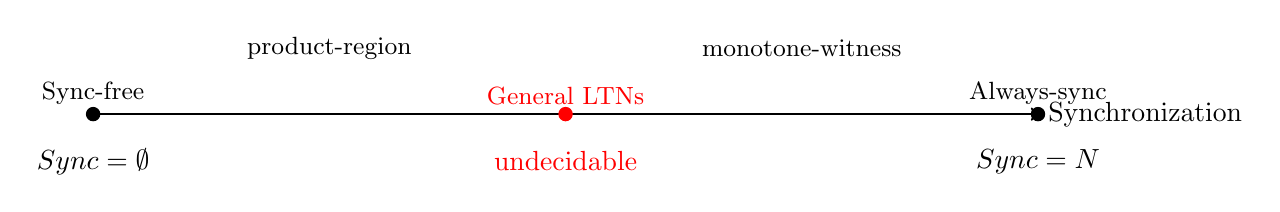
\begin{tikzpicture}[scale=1.2]
\draw[thick, ->] (0,0) -- (10,0) node[right] {Synchronization};
\node at (0,-0.5) {$\text{Sync} = \emptyset$};
\node at (10,-0.5) {$\text{Sync} = N$};
\filldraw (0,0) circle (2pt) node[above] {\small Sync-free};
\filldraw (10,0) circle (2pt) node[above] {\small Always-sync};
\filldraw[red] (5,0) circle (2pt) node[above] {\small General LTNs};
\node[red] at (5,-0.5) {undecidable};
\node at (2.5,0.7) {\small product-region};
\node at (7.5,0.7) {\small monotone-witness};
\end{tikzpicture}
\end{center}

\paragraph{Intermediate fragments.} What about LTNs where some nodes synchronize and others don't ($\emptyset \subset \text{Sync} \subset N$)? Two approaches:

\textbf{1. Quantitative restrictions (Chapter~\ref{chap:drift}):} Bound how much drift can accumulate, even with selective synchronization. If differences $t_p - t_q$ stay bounded, finite abstractions may still exist.

\textbf{2. Structural restrictions (Chapter~\ref{chap:connected}):} Require that control-flow structure prevents "problematic" patterns. For instance, demand that every cycle includes enough synchronization to prevent unbounded drift accumulation.

%-------------------------------------------------------------------------------

\section{Coming next}
\label{sec:fragments-coming-next}

This chapter established \PSPACE-completeness at the two extremes of
synchronization: when synchronization is absent, timing constraints remain
purely local and admit a product-region abstraction; when every node
synchronizes, every reachable location has a monotone witness run and
reachability reduces to timed-automata reachability.

\smallskip
In the next chapter we move to a genuinely intermediate regime: the
\emph{bounded-drift} fragment, where the deviation between agents' reference
times is globally bounded. We show how this quantitative restriction can be
exploited to recover a finite abstraction for reachability, and we analyze the
resulting complexity.


